% A4縦・1段組の学習用（教科書風）
\documentclass[dvipdfmx,paper=a4,fleqn,11pt]{jlreq}
\special{papersize=\the\paperwidth,\the\paperheight}

\usepackage[margin=20truemm]{geometry}
\usepackage[dvipdfmx]{graphicx}
\usepackage{amsmath,amssymb}
\usepackage{tikz}
\usepackage{pgfplots}
\usepackage{multicol}
\usepackage{etoolbox}
\usepackage{needspace}
\usepackage{bm}
\pgfplotsset{compat=1.18}
\usetikzlibrary{arrows.meta,calc,angles,quotes}

\linespread{1.08}

\AtBeginEnvironment{tikzpicture}{\vspace{3pt}}
\AfterEndEnvironment{tikzpicture}{\vspace{3pt}}

\preto{\section}{\needspace{0.35\textheight}}
\preto{\subsection}{\needspace{0.25\textheight}}

\ModifyHeading{section}{
  lines=1,
  before_space=14pt,
  after_space=6pt
}

\ModifyHeading{subsection}{
  lines=1,
  before_space=16pt,
  after_space=8pt
}

\title{物理基礎（丁寧解説版）}
\author{}
\date{}

\makeatletter
\renewcommand{\maketitle}{%
  \vspace*{-50pt}
  \begin{center}
    {\LARGE\bfseries \@title\par}
  \end{center}
  \vspace{4pt}
}
\makeatother

\newcommand{\formula}[1]{%
  \vspace{10pt}%
  \begin{center}{\large\bfseries\boldmath\(\displaystyle #1\)}\end{center}%
  \vspace{4pt}%
}

\newcommand{\dimcheck}[3]{%
  \begin{itemize}
    \item 左辺の次元: #1
    \item 右辺の次元: #2
    \item 判定: #3
  \end{itemize}
}

\newcommand{\bridge}[2]{%
  \vspace{4pt}
  \noindent\fbox{\parbox{0.97\linewidth}{%
  \textbf{次に進む準備}\par
  穴埋めで確認する語句: #1\par
  繰数で定着する計算: #2}}
  \vspace{4pt}
}

\begin{document}
\maketitle

\section{この教材の使い方（最初に読む）}

\subsection{3ステップ学習}
この単元は次の順で学ぶ。
\begin{enumerate}
  \item \textbf{テキストで理解}: 現象を図で見て、言葉と式をつなぐ。
  \item \textbf{穴埋めで整理}: キーワードと公式を短く確認する。
  \item \textbf{繰数で定着}: 計算と説明を何度か繰り返して身につける。
\end{enumerate}

\subsection{この単元で大事にすること}
\begin{itemize}
  \item ベクトルを「矢印」として毎回イメージする。
  \item 公式は暗記の前に意味を読む。
  \item 計算後は必ず単位と次元を確認する。
\end{itemize}

\begin{center}
\begin{tikzpicture}[scale=0.95,>=Stealth]
  \draw[rounded corners,fill=gray!10] (0,0) rectangle (3.7,1.2);
  \draw[rounded corners,fill=gray!10] (4.4,0) rectangle (8.1,1.2);
  \draw[rounded corners,fill=gray!10] (8.8,0) rectangle (12.5,1.2);
  \node at (1.85,0.6) {テキスト};
  \node at (6.25,0.6) {穴埋め};
  \node at (10.65,0.6) {繰数};
  \draw[->,very thick] (3.7,0.6) -- (4.4,0.6);
  \draw[->,very thick] (8.1,0.6) -- (8.8,0.6);
\end{tikzpicture}
\end{center}

\newpage

\section{ベクトルで物理量を見る}

\subsection{スカラー量とベクトル量を分ける}
\textbf{スカラー量}は大きさだけ、\textbf{ベクトル量}は大きさと向きをもつ。

\begin{center}
\begin{minipage}[t]{0.48\linewidth}
\vspace{0pt}
\centering
\textbf{スカラー量のイメージ}\par
\begin{tikzpicture}[scale=0.9]
  \node[draw,rounded corners,fill=gray!10,minimum width=3.7cm,minimum height=1.0cm] at (0,0) {$m=2\ \mathrm{kg}$};
  \node at (0,-0.9) {数値だけで決まる};
\end{tikzpicture}
\end{minipage}
\hfill
\begin{minipage}[t]{0.48\linewidth}
\vspace{0pt}
\centering
\textbf{ベクトル量のイメージ}\par
\begin{tikzpicture}[scale=0.85,>=Stealth]
  \draw[->,gray!60] (-0.5,0) -- (4.8,0) node[right] {$x$};
  \draw[->,gray!60] (0,-0.5) -- (0,3.2) node[above] {$y$};
  \draw[->,very thick,blue] (0,0) -- (3.4,2.0);
  \node[blue] at (2.1,1.6) {$\bm{v}$};
  \node at (2.1,-0.9) {向きと大きさが必要};
\end{tikzpicture}
\end{minipage}
\end{center}

\subsection{2次元ベクトルとの接続}
すでに学習した
\formula{\bm{a}=\begin{pmatrix}a_x & a_y\end{pmatrix}}
は、物理では「右方向成分」「上方向成分」をそのまま表す。

\textbf{読み方のコツ}
\begin{itemize}
  \item $a_x>0$ なら右向き、$a_x<0$ なら左向き
  \item $a_y>0$ なら上向き、$a_y<0$ なら下向き
\end{itemize}

\begin{center}
\begin{tikzpicture}[scale=0.95,>=Stealth]
  \draw[->,gray!60] (-1.2,0) -- (5.5,0) node[right] {$x$};
  \draw[->,gray!60] (0,-2.0) -- (0,3.2) node[above] {$y$};
  \draw[dashed,gray!65] (3.5,0) -- (3.5,2.0);
  \draw[dashed,gray!65] (0,2.0) -- (3.5,2.0);
  \draw[very thick,blue,->] (0,0) -- (3.5,2.0) node[midway,above left] {$\bm{a}$};
  \node at (3.5,-0.35) {$a_x$};
  \node at (-0.35,2.0) {$a_y$};
\end{tikzpicture}
\end{center}

\subsection{単位と次元をていねいに区別する}
単位は「m/s」などの書き方、次元は「$L/T$」などの量の種類である。

\begin{center}
\begin{tabular}{|c|c|c|}
\hline
物理量 & 単位 & 次元 \\\hline
速度 $\bm{v}$ & m/s & $L/T$ \\\hline
加速度 $\bm{a}$ & m/s$^2$ & $L/T^2$ \\\hline
力 $\bm{F}$ & N & $ML/T^2$ \\\hline
仕事 $W$ & J & $ML^2/T^2$ \\\hline
\end{tabular}
\end{center}

\textbf{注意}
\begin{itemize}
  \item km/h と m/s は単位が違うだけで、どちらも次元は $L/T$ で同じ。
\end{itemize}

\subsection{章末の理解チェック}
\begin{enumerate}
  \item 速度、質量、力をスカラー量とベクトル量に分類せよ。
  \item $\bm{a}=\begin{pmatrix}2 & -1\end{pmatrix}$ の向きを言葉で説明せよ。
  \item 単位と次元の違いを1文で説明せよ。
  \item 次元 $ML/T^2$ をもつ物理量を挙げよ。
\end{enumerate}

\bridge{スカラー量、ベクトル量、単位、次元}{分類問題、次元判定の基本問題}

\newpage

\section{速度と加速度を図で理解する}

\subsection{速度は「位置の変化」}
1秒ごとの位置を比べると、速いか遅いかが分かる。

\begin{center}
\begin{tikzpicture}[scale=0.95,>=Stealth]
  \draw[->,gray!60] (0,0) -- (12.5,0) node[right] {位置 $x$};
  \foreach \x/\t in {1/0,4/1,8/2,11/3} {
    \fill (\x,0) circle (2.2pt);
    \node[below] at (\x,-0.02) {$t=\t$ s};
  }
  \draw[thick,->] (1,0.35) -- (4,0.35);
  \draw[thick,->] (4,0.35) -- (8,0.35);
  \draw[thick,->] (8,0.35) -- (11,0.35);
\end{tikzpicture}
\end{center}

\textbf{Point:} 時間あたりの位置変化が速度である。

\formula{\bm{v}=\frac{\Delta \bm{x}}{\Delta t}}

\subsection{速さはベクトルの長さ}
速度ベクトル $\bm{v}=\begin{pmatrix}v_x & v_y\end{pmatrix}$ の速さは
\formula{|\bm{v}|=\sqrt{v_x^2+v_y^2}}
で求める。

\begin{center}
\begin{tikzpicture}[scale=0.9,>=Stealth]
  \draw[->,gray!60] (-0.4,0) -- (5.6,0) node[right] {$x$};
  \draw[->,gray!60] (0,-0.4) -- (0,4.6) node[above] {$y$};
  \draw[dashed,gray!65] (4,0) -- (4,3);
  \draw[dashed,gray!65] (0,3) -- (4,3);
  \draw[very thick,blue,->] (0,0) -- (4,3) node[midway,above left] {$\bm{v}$};
  \node at (2,-0.35) {$v_x=4$};
  \node at (-0.45,1.5) {$v_y=3$};
  \node at (2.2,1.9) {$|\bm{v}|=5$};
\end{tikzpicture}
\end{center}

\subsection{加速度は「速度の変化」}
\formula{\bm{a}=\frac{\Delta \bm{v}}{\Delta t}}

\textbf{意味を分解する}
\begin{itemize}
  \item $\Delta \bm{v}$: 速度ベクトルの差（向きも変わる）
  \item $\Delta t$: その変化にかかった時間
\end{itemize}

\begin{center}
\begin{tikzpicture}[scale=0.95,>=Stealth]
  \draw[->,gray!60] (-0.6,0) -- (6.2,0) node[right] {$x$};
  \draw[->,gray!60] (0,-0.6) -- (0,4.4) node[above] {$y$};
  \draw[very thick,blue,->] (0,0) -- (2.8,1.0) node[midway,below] {$\bm{v}_1$};
  \draw[very thick,teal!70!black,->] (0,0) -- (3.4,2.6) node[midway,above left] {$\bm{v}_2$};
  \draw[very thick,red,->] (2.8,1.0) -- (3.4,2.6) node[midway,right] {$\Delta\bm{v}$};
\end{tikzpicture}
\end{center}

\subsection{ディメンションで確認する}
\formula{\bm{a}=\frac{\Delta \bm{v}}{\Delta t}}
\dimcheck{$L/T^2$}{$(L/T)/T=L/T^2$}{一致}

\subsection{ゲーム場面で読み替える}
\begin{itemize}
  \item スティックを倒す: 速度の向きが変化する。
  \item 空中で方向転換: $\Delta\bm{v}$ が生まれ、加速度が発生する。
\end{itemize}

\subsection{章末の理解チェック}
\begin{enumerate}
  \item $\bm{v}=\begin{pmatrix}6 & 8\end{pmatrix}$ の速さを求めよ。
  \item $\Delta\bm{v}=\begin{pmatrix}4 & -2\end{pmatrix}$, $\Delta t=2$ s から $\bm{a}$ を求めよ。
  \item $\bm{a}=\Delta\bm{v}/\Delta t$ の左右次元が一致することを示せ。
  \item 空中で左入力したときの速度変化を言葉で説明せよ。
\end{enumerate}

\bridge{速度、速さ、加速度、速度差}{速さ計算、加速度計算、次元一致判定}

\newpage

\section{力と運動方程式をていねいに読む}

\subsection{力はベクトルとして合成する}
同時に複数の力があるとき、合力はベクトルの足し算で求める。

\formula{\bm{F}_{\mathrm{net}}=\bm{F}_1+\bm{F}_2+\cdots}

\begin{center}
\begin{tikzpicture}[scale=0.95,>=Stealth]
  \draw[->,gray!60] (-0.6,0) -- (6.0,0) node[right] {$x$};
  \draw[->,gray!60] (0,-0.6) -- (0,4.8) node[above] {$y$};
  \draw[very thick,black,->] (0,0) -- (3.2,0.0) node[midway,below] {$\bm{F}_1$};
  \draw[very thick,black,->] (0,0) -- (0.0,2.6) node[midway,left] {$\bm{F}_2$};
  \draw[very thick,teal!70!black,->] (0,0) -- (3.2,2.6) node[midway,above right] {$\bm{F}_{\mathrm{net}}$};
\end{tikzpicture}
\end{center}

\subsection{運動方程式を1行ずつ読む}
\formula{\bm{F}=m\bm{a}}

\begin{itemize}
  \item 力 $\bm{F}$ が大きいほど、加速度 $\bm{a}$ は大きくなりやすい。
  \item 質量 $m$ が大きいほど、同じ力でも加速度 $\bm{a}$ は小さくなる。
\end{itemize}

\begin{center}
\begin{tikzpicture}[scale=0.95,>=Stealth]
  \draw[rounded corners,fill=gray!10] (0,0) rectangle (3.3,2.2);
  \draw[rounded corners,fill=gray!10] (4.8,0) rectangle (8.1,2.2);
  \node at (1.65,1.8) {小さい質量};
  \node at (6.45,1.8) {大きい質量};
  \draw[very thick,->] (0.5,1.1) -- (2.8,1.1) node[midway,above] {$\bm{F}$};
  \draw[very thick,->,blue] (1.1,0.5) -- (2.9,0.5) node[midway,below] {$\bm{a}$ 大};
  \draw[very thick,->] (5.3,1.1) -- (7.6,1.1) node[midway,above] {$\bm{F}$};
  \draw[very thick,->,blue] (5.9,0.5) -- (6.8,0.5) node[midway,below] {$\bm{a}$ 小};
\end{tikzpicture}
\end{center}

\subsection{次元で式の正しさを検査する}
\formula{\bm{F}=m\bm{a}}
\dimcheck{$ML/T^2$}{$M\cdot L/T^2=ML/T^2$}{一致}

誤り例
\formula{\bm{F}=m\bm{v}}
\dimcheck{$ML/T^2$}{$M\cdot L/T=ML/T$}{不一致}

\subsection{作用反作用を図で確認する}
\begin{center}
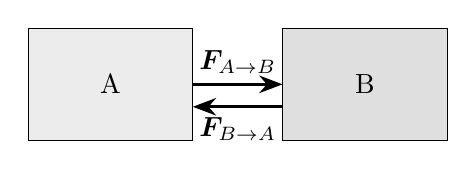
\begin{tikzpicture}[scale=0.95,>=Stealth]
  \draw[fill=gray!15] (1.0,0.5) rectangle (3.2,2.0);
  \draw[fill=gray!25] (4.4,0.5) rectangle (6.6,2.0);
  \node at (2.1,1.25) {A};
  \node at (5.5,1.25) {B};
  \draw[very thick,->] (3.2,1.25) -- (4.4,1.25) node[midway,above] {$\bm{F}_{A\to B}$};
  \draw[very thick,->] (4.4,0.95) -- (3.2,0.95) node[midway,below] {$\bm{F}_{B\to A}$};
\end{tikzpicture}
\end{center}

\textbf{Point:} 大きさは同じ、向きは反対。別々の物体にはたらく力なので打ち消し合わない。

\subsection{章末の理解チェック}
\begin{enumerate}
  \item $m=2$ kg, $\bm{a}=\begin{pmatrix}3 & 0\end{pmatrix}$ m/s$^2$ のとき $\bm{F}$ を求めよ。
  \item $\bm{F}=\begin{pmatrix}0 & -9.8\end{pmatrix}$ N, $m=1$ kg のとき $\bm{a}$ を求めよ。
  \item $\bm{F}=m\bm{a}$ の次元一致を示せ。
  \item 作用反作用を衝突の例で説明せよ。
\end{enumerate}

\bridge{合力、運動方程式、作用反作用、次元検査}{合力計算、F=ma計算、誤式判定}

\newpage

\section{仕事とエネルギーを図でつなぐ}

\subsection{仕事は「力と移動の重なり」}
仕事は、力が移動方向にどれだけ効いたかを表す。

\formula{W=\bm{F}\cdot\bm{d}=|\bm{F}||\bm{d}|\cos\theta}

\begin{center}
\begin{tikzpicture}[scale=0.95,>=Stealth]
  \draw[->,gray!60] (-0.6,0) -- (6.0,0) node[right] {$x$};
  \draw[->,gray!60] (0,-0.6) -- (0,3.8) node[above] {$y$};
  \draw[very thick,blue,->] (0,0) -- (4.0,0.0) node[midway,below] {$\bm{d}$};
  \draw[very thick,black,->] (0,0) -- (3.2,2.0) node[midway,above left] {$\bm{F}$};
  \draw (1.0,0) arc[start angle=0,end angle=32,radius=1.0];
  \node at (1.3,0.45) {$\theta$};
\end{tikzpicture}
\end{center}

\textbf{読み取り}
\begin{itemize}
  \item $\theta=0^\circ$ に近いほど、力は移動に効きやすい。
  \item $\theta=90^\circ$ のとき、理想化すると仕事は0。
\end{itemize}

\subsection{運動エネルギーと位置エネルギー}
\formula{K=\frac{1}{2}m|\bm{v}|^2}
\formula{U=mgh}

\begin{center}
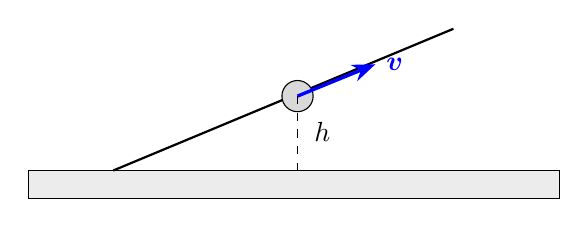
\begin{tikzpicture}[scale=0.9,>=Stealth]
  \draw[fill=gray!15] (0,0) rectangle (7.5,0.4);
  \draw[thick] (1.2,0.4) -- (6.0,2.4);
  \draw[fill=gray!30] (3.8,1.45) circle (0.22);
  \draw[->,very thick,blue] (3.8,1.45) -- (4.9,1.9) node[right] {$\bm{v}$};
  \draw[dashed] (3.8,1.45) -- (3.8,0.4);
  \node[right] at (3.9,0.95) {$h$};
\end{tikzpicture}
\end{center}

\textbf{場面ごとの見方}
\begin{itemize}
  \item 上にいるほど $U$ が大きい。
  \item 速く動くほど $K$ が大きい。
\end{itemize}

\subsection{次元で最終確認}
\formula{W=\bm{F}\cdot\bm{d}}
\dimcheck{$ML^2/T^2$}{$(ML/T^2)\cdot L=ML^2/T^2$}{一致}

\formula{K=\frac{1}{2}m|\bm{v}|^2}
\dimcheck{$ML^2/T^2$}{$M\cdot(L/T)^2=ML^2/T^2$}{一致}

\subsection{章末の理解チェック}
\begin{enumerate}
  \item $\bm{F}=\begin{pmatrix}10 & 0\end{pmatrix}$ N, $\bm{d}=\begin{pmatrix}4 & 3\end{pmatrix}$ m の仕事を求めよ。
  \item $m=2$ kg, $|\bm{v}|=4$ m/s のとき運動エネルギーを求めよ。
  \item $m=1$ kg, $g=9.8$ m/s$^2$, $h=2$ m のとき位置エネルギーを求めよ。
  \item $E=m|\bm{v}|$ がエネルギー式として不適切な理由を次元で説明せよ。
\end{enumerate}

\bridge{仕事、内積、運動エネルギー、位置エネルギー}{仕事計算、エネルギー計算、次元検査}

\newpage

\section{総まとめ（穴埋め・繰数へ接続）}

\subsection{このテキストで理解したこと}
\begin{enumerate}
  \item 物理量はスカラー量とベクトル量に分かれる。
  \item 速度と加速度はベクトルで表すと読みやすい。
  \item 力は合成でき、運動方程式 $\bm{F}=m\bm{a}$ で加速度とつながる。
  \item 仕事とエネルギーは内積と速さで表せる。
  \item 公式の正しさは次元で検査できる。
\end{enumerate}

\subsection{穴埋めで確認する項目}
\begin{itemize}
  \item 用語: スカラー量、ベクトル量、次元、合力、仕事
  \item 公式: $\bm{a}=\Delta\bm{v}/\Delta t$, $\bm{F}=m\bm{a}$, $W=\bm{F}\cdot\bm{d}$
  \item 単位と次元: m/s と $L/T$ などの対応
\end{itemize}

\subsection{繰数で定着する項目}
\begin{itemize}
  \item 速さ計算、加速度計算、合力計算
  \item 運動方程式の逆算（$F,m,a$ の3量）
  \item 仕事とエネルギー計算
  \item 誤った式の次元判定
\end{itemize}

\subsection{最後のセルフチェック}
\begin{enumerate}
  \item 自分で図を描いて、ベクトルの向きを説明できるか。
  \item 計算結果に単位を書けるか。
  \item 左辺と右辺の次元一致を確認したか。
\end{enumerate}

\end{document}
